% kapitel2.tex
\chapter{Background}
\label{chapter:kap2}
In this chapter, we are going to introduce the necessary background in generative modeling, with a focus on canonical exponential family distributions, Markov random fields, and the parameter estimation for these types of models.
Additionally, we will introduce the general notion of distributed learning and algorithms to sample from generative models.

As it is our goal to use aggregation methods on models obtained from distributed learners, we start by initially creating and training these models from observed data. 
We will then put this result in the context of distributed learning as the next step towards an aggregate model.
However, let us first define some basic concepts and notation, which are going to be used in this work.


\section{Notation}
    \label{sec:nota}
    Let us start by introducing tools and notations frequently encountered in probability theory and machine learning.
    This includes the definition of random variables, probability distributions, data, and parameters.
    A stochastic process is defined over random variables over a shared probability space, where expressions of random variables, the samples from a sample space are associated with a probability distribution. 
    We write $\mathbb{P}(X = x)$ for the probability of $X$ taking on value $x$.
    \begin{definition}{Random Variable}
        \label{def:randvar}
        Let $(\Omega, \mathcal{F}, \mathbb{P})$ be a probability space, where $\Omega$ is the domain, $\mathcal{F}$ is a $\sigma$-Algebra containing all possible outcomes and $\mathbb{P}: \mathcal{F} \rightarrow [0,1]$ is a probability measure defined on all possible outcomes.
        A Random Variable $X: \Omega \rightarrow \mathcal{X}$ is a measurable function defined over all possible outcomes of the probability space that maps these to the domain $\mathcal{X}$.

        Parametrized probability measures will be denoted $\mathbb{P}_{\vect{\theta}} (X = x)$, i.e., the probability of $X$ taking on some value $x$.
    \end{definition}

    Random vectors will be written in bold letters $\vect{X} = (X_1, X_2, \ldots, X_m)$, where again each entry in the vector is a random variable.
    The state-space of a random variable will be denoted as a cursive letter of that random variable e.g.$\mathcal{X}$ and the domain of a random vector likewise as $\vect{\mathcal{X}} = (\mathcal{X}_1, \mathcal{X}_2, \ldots, \mathcal{X}_m)$, where each $\mathcal{X}_i$ if the random variable is discrete, has a finite state-space.
    For example a six-sided die can be interpreted as univariate random variable with state-space $\mathcal{X} = \{1,2,3,4,5,6\}$, where each state has probability $\mathbb{P}(X=x) = 1/6$.
    Samples from a random variable $\vect{X}$  with state-space $\vect{\mathcal{X}}$ are denoted as lower case letters, e.g. $\vect{x} \in \mathcal{X}^m$ over an m-dimensional state-space.
    We express each element of a random variable in terms of a subscript, e.g., $\vect{X}_i$ or $\vect{X}_A$, where $A \subset\{1, \ldots, m\} $ addresses a subset of the dimensions.

    Then, let $\mathcal{D} = \{(\vect{x}^1, y^1), \ldots, (\vect{x}^n, y^n)\} \subset \mathbb{R}^m \times \mathbb{N}$ be a data set containing samples $\vect{x}^i \in \mathcal{X}^m$ from a m-variate random variable $\vect{X}$ and label domain $y^i \in \mathcal{Y}$, which can simply be expressed as an additional random variable $\vect{Y}$.
    Since label- and data space are not treated inherently different for generative modeling, we may also write $\mathcal{D} = \{\vect{x}^1, \ldots, \vect{x}^n\}$, where the labels are implicitly included.

    Furthermore let $\mathcal{D}_A$ denote a subset of samples for any indexing set $A\subset \{1, \ldots n\}$ and $\mathcal{D}_{\cdot B}$ be all samples from a subset of features indexed by $B \subset \{1, \ldots, m\}$.
    A subset of samples may also be referred to as rows and a subset of features as columns, when interpreting the data as a $n \times m$ matrix.  

    Parameters of a parametrized probability density function for canonical exponential families are noted as $\vect{\theta} \in \mathbb{R}^n$, while additional parameters will be explicitly introduced if necessary.
    Given a set of model parameters from distributed learners $\mathcal{M} = \{\vect{\theta}^1,  \ldots, \vect{\theta}^k\}$, each parameter vector $\vect{\theta}^i$ denotes the parameters obtained from the  $i^{th}$ learner, while $\vect{\theta_i}$ is the entry at position i$^{th}$ of a parameter vector.
    A multivariate gaussian normal distribution for example has parameters of the form $\vect{\theta} = (\vect{\mu}, \vect{\Sigma})$, with mean $\vect{\mu} \in \mathbb{R}^{n}$ and covariance matrix $\vect{\Sigma} \in \mathbb{R}^{n \times n}$.
    Additional notations for model parameters will be introduced if necessary.
    In the context of optimization and optimality, we assume $\vect{\theta}^*$ to be the true, unknown parameter vector.
    The global parameters vectors, i.e., the parameters obtained by a global model, which has access to all available data is denoted as  $\vect{\hat{\theta}}$.
    Finally, $\vect{\tilde{\theta}}$ denotes any local parameter vector and $\vect{\theta}^{i}$ the i$^{th}$ local parameter vector respectively.

    Now that we have defined so basic notation let us move on to the introduction of probabilistic graphical models, exponential families, and statistical inference.


\section{Probabilistic Graphical Models}
\label{sec:pgm}
Given a data set $\mathcal{D}$ our goal is to find a distribution $\mathbb{P}_{\vect{\theta}}$, such that the probability distribution matches the data distribution.
Probabilistic graphical models offer an interpretable visualization of random variables from a joint probability distribution and relationships between individual variables.
We assume that samples from features in $\mathcal{D}$ are realizations of random variables, which are then represented as nodes in a graph.
    \begin{definition}{Undirected Graph}
        Let $G=(V,E)$ be a graph with a set of elements $V$ called vertices and a set of edges $E \subseteq V \times V$ between pairs of vertices. 
        We exclude self-edges e.g. $(x,x)$ from this definition.

        The graph G is undirected if existing edges can be traversed in both directions, i.e., $(u,v) \in E \Leftrightarrow (v,u) \in E$.

        Given a vertex $v \in V$, $\mathcal{N}(v) = \{w \:\lvert\: w \in V, (v,w) \in E\}$ is the set of neighbors in G, i.e., all nodes w that have an edge between themselves and v.

        A path $P = \{v_1, \ldots, v_p\}$ is a series of vertices, where two subsequent vertices in the series have an existing edge in G. 
        A unique path is a path, where each vertex of G appears at most once in the path.
        If $v_1 = v_p$, the path is not unique and P is called a cycle.
    \end{definition}
In order to determine such a distribution and estimate its parameters we first have to establish the structure of the model, i.e., perform feature selection and establish relationships between random variables.
Our goal is to find a probability distribution $\mathbb{P}_{\vect{\theta}}$ and its parameters $\vect{\theta}$, such that the probability distribution $\mathbb{P}_{\vect{\theta}}$ is optimal \wrt to the observed data.
%Conditional independence
When all random variables are statistically independent of each other  we obtain the joint probability distribution
\begin{equation}
    \mathbb{P}_{\vect{\theta}}(\vect{X} = \vect{x}) = \prod_{i=1}^m \mathbb{P}_{\vect{\theta}}(\vect{X}_i = \vect{x}_i)
\end{equation}
by factorization over the individual probabilities for each random variable.
In practice random variables are rarely fully independent and thus the assumption of statistical independence does not perform well.
Hence, it is vital to properly capture dependencies between random variables.
This however increases the model's complexity up to a point where it is not computationally feasible anymore to perform parameter estimation.
For general graphs with arbitrary conditional independencies, no closed form solution is known for parameter estimation. 
An exception to this problem are special types of graphs such as trees or polytrees, for which closed form solutions exist.\todo{cite}
\begin{definition}{Conditional Independence}
    Let $\vect{X}, \vect{Y}$ be two random variables. Two random variables are independent,  $\vect{X} \independent \vect{Y}$, if and only if
    \begin{equation}
        \begin{split}
        \forall \vect{x} \in \mathcal{X}, \vect{y} \in \mathcal{Y}:  \; \mathbb{P}(\vect{X} = x \lvert \vect{Y} = y) &= \frac{\mathbb{P}(\vect{X} = x , \vect{Y} = y)}{\mathbb{P}(\vect{Y} = \vect{y})} \\
        &=  \frac{\mathbb{P}(\vect{X} = x) \mathbb{P}(\vect{Y} = \vect{y})}{\mathbb{P}(\vect{Y} = \vect{y})}.  \\
        \end{split}
    \end{equation} 
    The joint probability is equal to the product of the individual probabilities for the all elements in the state-space of either random variable.
    This definition is extended by the notion of conditional independence. 
    Two random variables are called conditionally independent if the factorization is independent given a third random variable $\vect{Z}$, that is
    \begin{equation}
        \forall \vect{x} \in \mathcal{X}, \vect{y} \in \mathcal{Y}: \mathbb{P}(\vect{X} = x , \vect{Y} = y \lvert \vect{Z} = \vect{z}) =   \mathbb{P}(\vect{X} = x \lvert \vect{Z} = \vect{z}) \mathbb{P}(\vect{Y} = y \lvert \vect{Z} = \vect{z})
    \end{equation}
    which will be written as $\vect{X} \independent \vect{Y} \lvert \vect{Z}$.

    \fig \ref{fig:condind} showcases an example based on three nodes from \fig \ref{fig:data}, which are connected by two edges. 
    When $X_s$ is fully observed $X_r$ and $X_w$ are independent of each other as no other path with unobserved random variables between them exists, we then write $X_r \independent X_w \lvert X_s$.   
    \begin{figure}[H]
    \center
    \begin{tikzpicture}
        \Vertex[x=0,y=0,color=tugreen,opacity=0.5,label=r, size=1, shape=circle]{r}
        \Vertex[x=2,y=0,color=tuorange,opacity=0.5,label=s, size=1, shape=circle]{s}
        \Vertex[x=4,y=0,color=tugreen,opacity=0.5,label=w, size=1, shape=circle]{w}
        \Edge[](r)(s)
        \Edge[](s)(w)
        \end{tikzpicture}
    \caption[Conditional Independence of Random Variables]{Minimal example for conditional independence consisting of a graph with three vertices and two edges. The random variable $X_r$ is conditionally independent of $X_w$ when $X_s$ is observed}
    \label{fig:condind}
\end{figure}        

\end{definition}

% Capturing Dependencies
%Let $\vect{X}$ be a random vector as defined in \sect \ref{sec:nota}. 
%Each element $X_i \in \vect{X}$ corresponds to a dimension of the random vector.
%The straightforward approach is to assume all entries to be statistically independent. 
%We may then simply estimate the parameters of a probability distribution individually for each random variable in $\vect{X}$, disregarding possible dependencies.
%This generally leads to worse overall estimates as the model can not capture existing dependencies between random variables.
%With probabilistic graphical models we can express dependencies between random variables in terms of edges in a graph. 
%Having the tools to model and express conditional independencies in such a way allows us to create more flexible and possibly more fitting distributions for our data $\mathcal{D}$.

\begin{figure}
    \center
    \begin{tikzpicture}
        \Vertex[x=0.5, y=0.5,color=white,opacity=0.5,label=p, size=1, shape=circle]{p}
        \Vertex[x=-1,y=3,color=white,opacity=0.5,label=q, size=1, shape=circle]{q}
        \Vertex[x=2,y=2.5,color=white,opacity=0.5,label=r, size=1, shape=circle]{r}
        \Vertex[x=4,y=4,color=white,opacity=0.5,label=s, size=1, shape=circle]{s}
        \Vertex[x=2.5,y=6.5,color=white,opacity=0.5,label=t, size=1, shape=circle]{t}
        \Vertex[x=5.5,y=1.75,color=white,opacity=0.5,label=u, size=1, shape=circle]{u}
        \Vertex[x=7.5,y=4,color=white,opacity=0.5,label=v, size=1, shape=circle]{v}
        \Vertex[x=7.5,y=6.5,color=white,opacity=0.5,label=w, size=1, shape=circle]{w}
        \Edge[](q)(r)
        \Edge[](p)(r)
        \Edge[](r)(s)
        \Edge[](w)(s)
        \Edge[](u)(s)
        \Edge[](t)(s)
        \Edge[](v)(s)
        \end{tikzpicture}
    \caption[Independence Structure of a Graph G with 8 Nodes]{Graph G=(V,E) with m=8 random variables from a dataset $\mathcal{D}$ with eight features and samples $\vect{x} = (x_p, x_q, x_r, x_s, x_t, x_u, x_v, x_w) \in \mathbb{R}^8$. The conditional independence structure is given by the edges of the graph. In this case, the graph is a tree, but independence structures are generally not limited to trees.}
    \label{fig:data}
\end{figure}

%Graph representation 
We introduce a random variable for each feature in $\mathcal{D}$ while treating the observed data as the result of a stochastic process.
Given a graph $G=(V,E)$, each vertex represents a single random variable and each edge between two vertices represents conditional independence. 
\fig \ref{fig:data} shows the graph representation $G=(V,E)$ of a such distribution for a graph with eight vertices. 
Each vertex $ v \in V$ indexes a random variable $X_v$.
Our goal is now to estimate the joint probability distribution given the graph G with established conditional independencies.
Parameter estimation and other operations associated with probabilistic graphical models are NP-Hard~\cite{cooper1990computational}.
%This is a direct result of the requirement to compute the marginal distribution in order to perform inference.
%This requires summing over all possible states for all random variables that are fully dependent on each other, which is the set of all maximal cliques in the graph, as we will later see.
However, algorithms for general graphs exist, which allow us to find an approximate solution in order to perform parameter estimation and inference tasks.

% Probability Dist. Factorization
A large number of well-known distributions, such as the normal distribution or exponential distribution are from a class of distribution called the exponential family.
Probability distributions from the exponential family can be expressed as a product of a normalizer and some non-negative function $\psi: \mathcal{X}^m \rightarrow \mathbb{R}_+$ usually called potential function:
\begin{equation}
    \label{eq:probpot}
    \mathbb{P}(\vect{X} = \vect{x}) = \frac{1}{Z} \psi(\vect{x}),
\end{equation}
where $Z$, the partition function ensures that the probability distribution properly sums to one.
If all entries in $\vect{X}$ are independent from each other we can write $\mathbb{P}(\vect{X} = \vect{x}) = \frac{1}{Z} \prod_{i=1}^m \psi_i(x_i)$ as the probability of a set of independent random variables is the product of each individual probability.
%\begin{example}{Normal Distribution}
%    For a multivariate normal distribution with mean $\vect{\mu}$ and covariance matrix $\vect{\Sigma}$
%    \begin{equation}
%        \mathcal{N}(\vect{x}; \vect{\mu}, \vect{\Sigma}) = \frac{1}{\sqrt{2 \pi \abs{\Sigma}}} \cdot \exp\bigg(-\frac{1}{2} (\vect{x} - \vect{\mu})^T \Sigma^{-1}(\vect{x} - \vect{\mu}))\bigg)
%    \end{equation}
%    we can express the normal distribution in terms of partition and potential function as follows
%    \begin{equation}
%        Z = \sqrt{2 \pi \abs{\Sigma}}, \quad \psi(\vect{x}) = \exp\bigg(-\frac{1}{2} (\vect{x} - \vect{\mu})^T \Sigma^{-1}(\vect{x} - \vect{\mu}))\bigg).
%    \end{equation}
%    Here the partition $Z$ only depends on the covariance matrix and the potential function is expressed in terms of the model parameters $\vect{\mu}, \vect{\Sigma}$
%    \label{ex:normdist}
%\end{example}
%After estimating the parameters for each distribution and device, we employ an aggregation mechanic to create a composite model.
%Distributed integer probabilistic graphical models \cite{piatkowski2019distributed} have recently been considered by Piatkowski.
%In this specific scenario the models were aggregated using the average over all local models.
%Other existing aggregation mechanics are discussed in section.
%Additionally we need to define a stopping criterion where every device will stop sending messages to other devices, which means we require some kind of convergence.
%This is usually the case when most devices have a similar local model.
%In the following we will consider existing work on that specific research area and then lay out the necessary steps and challenges for the thesis.

%Capturing Statistical Independencies
However, in practice, random variables are rarely fully independent of each other, while they also may not be completely dependent on all other random variables.
This is captured by establishing conditional independencies between random variables.
If the graph satisfies a set of properties, called the Markov Properties, the graph is a Markov Random Field and the joint probability distribution can be expressed in a convenient way.

\subsection{Markov Random Fields}
%TODO Graph Representation
%MRF Definition
Markov Random Fields are undirected graphs used to express conditional independencies between random variables. 
Markov Random Fields are probabilistic graphical models, that represent the joint probability of a random variable $(\vect{X}_v), \; v \in V$ and state-space $\mathcal{X}_v$ \wrt to the vertices and their conditional independencies through edges of the graph. 

For $\vect{X}$ to be considered a Markov Random Field \wrt G the Markov Properties, have to hold:

%MRF Properties
\subsubsection*{Markov Properties}
Probabilistic graphical models are considered Markov Random Fields if G is undirected and the three Markov properties hold for any set of random variables indexed by the vertices of G, $\vect{X} = \{X_v\}, v \in V$

\paragraph*{Pairwise Markov Property}
Two random variables $X_u, X_v$ are independent given all other random variables if they are not adjacent, i.e. $\not\exists (u,v) \in E$ :
\begin{equation}
    X_u \independent X_v \lvert X_{V \setminus\{u,v\}}
\end{equation}

\paragraph*{Local Markov Property}
Given a random variable $X_v$ it is independent of all other variables if all neighbors are observed 
\begin{equation}
    X_v \independent X_{V\setminus (v \cup \mathcal{N}(v))} \lvert X_{\mathcal{N}(v)},   
\end{equation}
where $\mathcal{N}: V \rightarrow V$ is the Markov Blanket of a node $v \in V$, i.e., the neighbors of $v$ such that $u \in \mathcal{N}(v) \Leftrightarrow (v,u) \vee (u,v) \in E$.

\paragraph*{Global Markov Property}
Let $A, B \subset V, A \cap B = \emptyset$ be two subsets of vertices from G. 
These subsets are independent if, given a third subset $C$, there exists no path from $A$ to $B$ that contains unobserved variables, i.e., all paths contain at least one variable from $C$:

\begin{equation}
    X_A \independent X_B \lvert X_C
\end{equation}

Instead of obtaining the joint probability over all random variables simultaneously we can express \eq~\ref{eq:probpot} as a factorization over cliques given that $\vect{X}$ satisfies the Markov properties. 

\paragraph*{Clique Factorization}

A clique is a special subset of nodes $C \subseteq V$ such that, $\forall u,v,  \in C, u \neq v: \exists (u,v) \in E$ there exists an edge in $E$ between all nodes in $C$, i.e., the subset of nodes is fully connected.
Now let $\mathcal{C}$ be set set of maximal cliques, i.e., the set of cliques that are not included in any other clique or formally 
\begin{equation}
    \forall C_i, C_j \in \mathcal{C},\; i \neq j  : C_i \not\subset C_j,\; C_j \not\subset C_i,\; C_i \neq C_j
\end{equation}
there exists no such pair of cliques in $\mathcal{C}$ such that either one is a true subset or the other.
This is not to be confused with the maximum clique, which is the largest clique of the graph $G$, i.e. $\max \mathcal{C} = \max \{\abs{\mathcal{C}_1}, \ldots, \abs{C_n}\}$ the clique with maximum cardinality.

If the Markov properties hold for $\vect{X}$ , we can express the joint probability distribution as factorization over the set of maximal cliques.
This allows us to split the potentials into smaller clique-based terms and compute them individually. 
We assign a potential function $\psi_C: \mathcal{X}_C \rightarrow \mathbb{R}$ to every clique in the graph.

\begin{equation}
        \mathbb{P}(\vect{X}=\vect{x}) = \frac{1}{Z} \cdot \psi(\vect{x})= \frac{1}{Z} \cdot \prod_{C \in \mathcal{C}} \psi_C(\vect{x}_C)
\end{equation},
where $Z$ is the normalizer of the probability density function, which ensures that $\mathbb{P}$  properly sums to one:

\begin{equation}
    \frac{1}{Z} \sum_{\vect{x}\in \mathcal{\vect{X}}} \prod_{C \in \mathcal{C}} \psi_C(\vect{x}_C) = 1. 
\end{equation}

The partition function $Z$ is then obtained by summing over the product of all maximal cliques in the graph for all possible states
\begin{equation}
    Z = \sum_{x\in \mathcal{X}} \prod_{C \in \mathcal{C}} \psi_C(\vect{x}_C).
\end{equation}
Positive potential functions with discrete state-space $\mathcal{X}_C$ can be expressed as inner product of parameters $\vect{\theta}_C \in \mathbb{R}^{\abs{\mathcal{X}_C}}$ and sufficient statistic $\phi_C: \mathcal{X}_C \rightarrow \mathbb{R}^{\abs{\mathcal{X}_C}}$ 
\begin{equation}
    \psi_C(\vect{x}_c) = \exp(\inner{\vect{\theta}_C}{\phi_C(\vect{x})}).
\end{equation}
We obtain the complete parameter vector and sufficient statistics by simply concatenating the individual results from each clique in order of appearance, which is usually determine by the order of edges in $E$.
The dimensionality of $\vect{\theta}$ is then given by $d = \sum_{C \in \mathcal{C}} \abs{\mathcal{X}_C}$ the sum over all clique state-spaces.
In order to guarantee independence from the data$\mathcal{D}$,  $\phi(\mathcal{D})$ has to be a sufficient statistic for $\vect{X}$ \wrt $\mathcal{D}$.
\paragraph*{Sufficiency}
    A function $\phi$  is a sufficient statistic of random variable $\vect{X}$ if the data is conditionally independent of the model parameters given $\phi$, that is if and only if $\vect{\theta}\independent \mathcal{D} \:\lvert\: \phi(\mathcal{D})$ the data and parameters are conditionally independent given $\phi$.
    The choice of $\phi: \vect{\mathcal{X}} \rightarrow \mathbb{R}^d$ directly determines the shape of  $\mathbb{E}_{\mathbb{P}}[\phi(x)]$.
    Let $C \in \mathcal{C}(G)$, be a clique in the set of maximum cliques of a graph G and let further
    $\phi_C: \vect{\mathcal{X}_C} \rightarrow \mathbb{R}^{\abs{\mathcal{X}_C}}$ be the sufficient statistic for that clique.
    Then if the domain of $\phi$ is binary, i.e., $\phi_C : \mathcal{X}_C \rightarrow \{0,1\}^{\abs{\mathcal{X}_C}}$ it is easy to see that  $\mathbb{E}_{\mathbb{P}}[\phi_C(x_C)_i] = P(\phi_C(\vect{x_C})_i = 1)$, since
    \begin{equation}
        \mathbb{E}_{\mathbb{P}}[\vect{X}] = 0 \cdot \mathbb{P}(\vect{X} = 0) + 1 \cdot \mathbb{P}(\vect{X}= 1) = \mathbb{P}(\vect{X} = 1), \quad \mathcal{X} \in \{0,1\}.
    \end{equation}
    Thus, the expectation is equal to the probability that a we observe a one in state $i$.
    In this case the sufficient statistics generated by $\phi_C$ are overcomplete, as we map each clique state to a binary vector, where only a single entry is one, while all other entries in that particular clique are zero.  

    
    \subsection{Exponential Families}
    \label{ssec:expf}
    One important result is that from the space of all feasible distributions $\mathcal{P}$, which fit the data $\mathcal{D}$, the canonical exponential family is the distribution that contains the most information \wrt the Shannon Entropy:
    \begin{equation}
    \max_{\mathbb{P}\in \mathcal{P}} \quad  H(\mathbb{P}) = - \sum_{x\in\mathcal{X}} \mathbb{P}(x) \log \mathbb{P}(x).
    \end{equation}

    The probability distribution

    \begin{equation}
        \mathbb{P}(X) = \exp(\inner{\vect{\theta}}{\vect{\phi_i(x)}} - A(\theta)),
    \end{equation}
    is the maximizer for the entropy $H(\mathbb{P})$.
    In order to find the optimal distribution, we additionally need to estimate the parameter $\vect{\theta}$ of $\mathbb{P}(X)$.

    Let us start with the definition of Shannon Entropy and why it is necessary to introduce some notion of optimality when it comes to finding a distribution which fits our observed data $\mathcal{D}$.
    The approach presented here follows the intuition presented by Wainwright and Jordan \cite{wainwright2008graphical}.

    We want to find the distribution $\mathbb{P}$ from the space of all probability distributions $\mathcal{P}$, that fits the data  $\mathcal{D}$ the most.
    However,  there are many such distributions $\mathbb{P} \in \mathcal{P}$ that satisfy this condition. 
    Let $\phi: \vect{\mathcal{X}}  \rightarrow \{0,1\}^d$ be the sufficient statistics of $\mathcal{D}$, that maps observations to a binary vector. 
    We then want to find a distribution such that:
    \begin{equation}
        \label{eq:expecval}
        \mathbb{E}_P[\phi(X)] = \tilde{\mathbb{E}}_{\mathcal{D}}[\phi(X)], 
    \end{equation}
    for every feature in $\vect{\mathcal{X}}$ the expectation of the probability distribution matches the expectation of the data set.

    We can find the best distribution \wrt the Shannon Entropy by maximizing a constrained optimization problem with equality constraints from \eq\ref{eq:expecval}:
    \begin{equation}
        \label{eq:entropy}
        \begin{split}
            \max_{P\in \mathcal{P}} \quad & H(P) = - \sum_{x\in\mathcal{X}} P(x) \log P(x) \\
            s.t. \quad & \mathbb{E}_P[\phi_(X)_d] = \tilde{\mathbb{E}}_{\mathcal{D}}[\phi(X)_d]  \; \forall d\\
            & \sum_{x\in \mathcal{X}} p(x) = 1.
        \end{split}
    \end{equation}
    Now let $\tilde{\mathbb{E}}_{\mathcal{D}}[\phi(X)] = \tilde{\vect{\mu}}$ and $\mathbb{E}_P[\phi_(X)] = \vect{\hat{\mu}}$.
    We can omit the inequality constraints for $p(x) \geq 0$ as it turns out that these constraints are redundant. 
    In order to optimize this constrained problem, we first introduce Lagrange multipliers to express equation \ref{eq:entropy} as an unconstrained optimization problem and turn the maximization into a minimization by multiplying the objective by minus one.
    We then obtain an unconstrained minimization problem with a set of additional variables $\vect{\theta}$
    \begin{equation}
        \min_{\mathbb{P}\in \mathcal{P}, \vect{\theta}, \vect{\theta_0} } \mathcal{L}(\mathbb{P}, \vect{\theta}, \theta_0) = \sum_{x\in\mathcal{X}} \mathbb{P}(x) \log \mathbb{P}(x) + \sum_{i=1}^d \theta_i (\tilde{\mu}_d - \sum_{x \in \mathcal{X}} \mathbb{P}(x) \phi_i(x)) + \theta_0 \sum_{x\in\mathcal{X}} \mathbb{P}(x) -1.
    \end{equation}
    One Lagrange multiplier is introduced for each constraint resulting in a total of $d+1$ Lagrange multipliers.
    We then compute the derivative of \eq\ref{eq:entropy} \wrt $P(x)$ :
    \begin{equation}
        \begin{split}
        \frac{\partial \mathcal{L}}{\partial \mathbb{P}} =  \frac{\partial}{\partial \mathbb{P}} \sum_{x\in\mathcal{X}} \mathbb{P}(\vect{x}) \log \mathbb{P}(\vect{x}) &+ \sum_{i=1}^d \theta_i (\tilde{\mu}_i - \sum_{x \in \mathcal{X}} \mathbb{P}(\vect{x}) \phi_i(\vect{x})) + \theta_0 \sum_{x\in\mathcal{X}} \mathbb{P}(\vect{x}) -1 \\ 
        &= 1 + \log \mathbb{P}(X) - \sum_{i=1}^d \theta_i  \phi_i(\vect{x}) + \theta_0 = 0 \\
        \log \mathbb{P}(\vect{x}) &=  \sum_{i=1}^d \theta_i  \phi_i(\vect{x}) - \theta_0 - 1 \\
        \mathbb{P}(\vect{x}) &= \exp{(\langle\vect{\theta}, \vect{\phi_i(\vect{x})} \rangle - \theta_0 - 1)} \\
    \end{split}
    \end{equation}

    and it follows that the objective function reaches its optimum when 
    \begin{equation}   
        \mathbb{P}(\vect{x}) = \exp{(\inner{\vect{\theta}}{\vect{\phi_i(\vect{x})}} - \theta_0 - 1)} = \mathbb{P}_{\vect{\theta}}(\vect{x})
    \end{equation} 
    and with setting $\theta_0 = -1 + A(\theta) $ we obtain the form of the canonical exponential family

    \begin{equation}
        P(\vect{x}) = \exp{(\langle\vect{\theta}, \vect{\phi_i(x)} \rangle - A(\theta))},
    \end{equation}
    where $A(\theta) = \log \sum_{\vect{x}\in \vect{\mathcal{X}}} \exp(\inner{\vect{\theta}}{\phi(\vect{x})})$ is the log partition function, the normalizer of the probability distribution, ensuring that the second set of constraints from \eq\ref{eq:entropy} is not violated.
    
    The remaining to maximize the entropy is to estimate the Lagrange multipliers $\vect{\theta}$, which are simultaneously the parameters of the canonical exponential family.

    \subsection{Training}
    \label{ssec:train}

    Now that we know, the type of  probability distribution that maximizes the entropy we have to determine the parameters $\vect{\theta} \in \Theta$, where $\Theta = \{\vect{\theta} \;\lvert A(\vect{\theta}) < \infty\} \subset \mathbb{R}^d$ is the set of feasible solutions.
    Using the gradient descent as first order iterative optimization method for a function $f: \mathbb{R}^d \rightarrow \mathbb{R}$, we can find the optimum by updating the parameters in an iterative fashion:
    \begin{equation}
        \label{eq:gradesc}
        \vect{\theta}^{t+1} = \vect{\theta}^{t} + \alpha \nabla f(\vect{\theta}^{t}).
    \end{equation}

    Note that in \eq\ref{eq:gradesc} the index $t+1$ does refer to an update of $\vect{\theta}$ and not the t-th model.
    Going forward we will use the index $t$ when referring to updates of parameters or models. 
    The choice of $f$ is usually the likelihood function
    \begin{equation}
        \label{eq:likelihood}
        \mathcal{L}(\vect{\theta} ; \mathcal{D}) = \arg\max_{\vect{\theta}}\prod_{\vect{x} \in \mathcal{D}}  \mathbb{P}_{\vect{\theta}}(\vect{X} = \vect{x}),
    \end{equation}
    which is a direct result of applying the Bayes' Rule to the posterior probability
    \begin{equation}
        \arg\max_{\vect{\theta}} \; \mathbb{P}(\vect{\theta} \lvert \mathcal{D}) = \arg\max_{\vect{\theta}} \; \frac{\mathbb{P}(\mathcal{D} \lvert \vect{\theta}) \mathbb{P}(\vect{\theta})}{\mathbb{P}(\mathcal{D})} \propto   \arg\max_{\vect{\theta}} \; \mathbb{P}(\mathcal{D} \lvert \vect{\theta}) \mathbb{P}(\vect{\theta}).
    \end{equation}
    Assuming a uniform prior distribution $\mathbb{P}(\vect{\theta})$ we obtain the model parameters $\vect{\theta}$ by maximizing the likelihood $\mathbb{P}(\mathcal{D} \lvert \vect{\theta})$.

    It is convenient to reformulate the problem as minimization instead of  maximization by multiplying the objective by minus one. 
    Furthermore, we apply the logarithm to the objective, which preserves the quality of the solution, while being numerically more stable.
    We then obtain the following minimization problem
    \begin{equation}
        \label{eq:likelihood:log}
        \ell(\vect{\theta} ; \mathcal{D}) = \arg\min_{\vect{\theta}} \; - \sum_{\vect{x} \in \mathcal{D}}  \log \mathbb{P}_{\vect{\theta}}(\vect{X} = \vect{x}).
    \end{equation}

    Additionally, when optimizing via first-order methods such as gradient descent, it is advantageous to use the average log-likelihood
    \begin{equation}
        \label{eq:likelihood:expfam}
        \begin{split}
        \ell(\vect{\theta}, \mathcal{D}) &= - \frac{1}{\abs{\mathcal{D}}} \sum_{\vect{x} \in \mathcal{D}} \log \mathbb{P}_{\vect{\theta}}(x)\\
        &= - \frac{1}{\abs{\mathcal{D}}} \sum_{\vect{x} \in \mathcal{D}} \inner{\vect{\theta}}{\phi(x)} - A(\vect{\theta})
    \end{split}
    \end{equation}
    instead as this formulation yields more stable results with first-order methods.
    This is due to the gradient of the likelihood increasing in value as the sample size increases, which causes us to take larger steps towards the gradient for larger $n$.
    Averaging with the sample size prevents this issue.

    Now computing the first derivative of the likelihood \wrt $\vect{\theta}$ and setting it to zero we obtain
    \begin{equation}
        \label{eq:likelihood_der}
        \begin{split}
            \frac{\partial \ell(\vect{\theta}, \mathcal{D})}{\partial \vect{\theta}} &=  \frac{\partial}{\partial \vect{\theta}}  - \frac{1}{\abs{\mathcal{D}}} \sum_{\vect{x} \in \mathcal{D}} \inner{\vect{\theta}}{\phi(x)} + A(\vect{\theta})\\
            &= - \frac{1}{\abs{\mathcal{D}}}  \sum_{\vect{x} \in \mathcal{D}} \phi(x) +  \frac{\partial}{\partial \vect{\theta}}  A(\vect{\theta}) \\
            &= - \frac{1}{\abs{\mathcal{D}}}  \sum_{\vect{x} \in \mathcal{D}} \phi(x) +  \frac{\partial}{\partial \vect{\theta}}  \log \sum_{\vect{x} \in \vect{\mathcal{X}}} \exp(\inner{\vect{\theta}}{\phi(\vect{x})})\\
            &= - \frac{1}{\abs{\mathcal{D}}}  \sum_{\vect{x} \in \mathcal{D}} \phi(x) +  \frac{1}{Z(\vect{\theta})}\frac{\partial}{\partial \vect{\theta}}  \sum_{\vect{x} \in \vect{\mathcal{X}}} \exp(\inner{\vect{\theta}}{\phi(\vect{x})})\\
            &= - \frac{1}{\abs{\mathcal{D}}}  \sum_{\vect{x} \in \mathcal{D}} \phi(x) +  \frac{1}{Z(\vect{\theta})} \sum_{\vect{x} \in \vect{\mathcal{X}}}  \frac{\partial}{\partial \vect{\theta}}  \exp(\inner{\vect{\theta}}{\phi(\vect{x})})\\
            &= - \frac{1}{\abs{\mathcal{D}}}  \sum_{\vect{x} \in \mathcal{D}} \phi(x) +  \frac{1}{Z(\vect{\theta})} \sum_{\vect{x} \in \vect{\mathcal{X}}} \exp(\inner{\vect{\theta}}{\phi(\vect{x})}) \frac{\partial}{\partial \vect{\theta}}  \inner{\vect{\theta}}{\phi(\vect{x})}\\
            &= - \frac{1}{\abs{\mathcal{D}}}  \sum_{\vect{x} \in \mathcal{D}} \phi(x) +  \frac{1}{Z(\vect{\theta})} \sum_{\vect{x} \in \vect{\mathcal{X}}} \exp(\inner{\vect{\theta}}{\phi(\vect{x})}) \phi(\vect{x})\\
            &= - \frac{1}{\abs{\mathcal{D}}}  \sum_{\vect{x} \in \mathcal{D}} \phi(x) + \sum_{\vect{x} \in \vect{\mathcal{X}}} \exp(\inner{\vect{\theta}}{\phi(\vect{x})} - A(\vect{\theta})) \phi(\vect{x})\\
            &= - \frac{1}{\abs{\mathcal{D}}}  \sum_{\vect{x} \in \mathcal{D}} \phi(x) + \sum_{\vect{x} \in \vect{\mathcal{X}}} \mathbb{P}_{\vect{\theta}}(\vect{X} = \vect{x}) \phi(\vect{x})\\
            &=  - \tilde{\mathbb{E}}_{\mathcal{D}}[\phi(x)] + \mathbb{E}_{\mathbb{P}}[\phi(x)]
        \end{split}
    \end{equation}
    which is the difference between the expected value of the probability distribution $\mathbb{P}$ and the empirical expectation, i.e., the average sufficient statistics implying that the optimum is achieved when empirical expectation and the distribution's expectation are equal.

    Unfortunately, evaluating the gradient requires us to compute the log partition function $A(\vect{\theta})$, where we have to sum over all possible states.
    This problem is known to be \#P-Complete, i.e., there exists no algorithm for efficiently computing the log partition other than brute force evaluation.
    However, it is possible to find an exact solution in polynomial time if the graph structure is a tree or polytree.
    Sum-Product message-passing algorithms on trees for example allow us to obtain an exact solution in polynomial time, while there are also algorithms for computing the log partition on a graph with bounded treewidth\cite{berg2014learning}.

    The problem of computing probabilities and the log partition function or partition function of a probability density is also known as inference.
    Here we will focus on inference where the graph G is a tree, which generally allows us to perform exact inference in polynomial time using sum-product message-passing algorithms such as Belief Propagation.

    Before introducing the means to perform inference, we will first showcase some additional useful properties of the log partition function and canonical exponential family representation.
    
    \paragraph*{Log Partition Function}
    For second-order methods such as Newton's Method the second derivative of the likelihood \wrt $\vect{\theta}$ may also be of interest.
    It can be shown (see for example \cite{piatkowski2018exponential}), that the second derivative of the log-likelihood is simply the second derivative of the log partition function :

    \begin{equation}
        \label{eq:sparsefish}
        \begin{split}
        \frac{\partial^2 A(\vect{\theta})}{\partial \vect{\theta}_i \partial \vect{\theta}_j} &= \mathbb{E}[\phi(\vect{X})_i \phi(\vect{X})_j] - \mathbb{E}[\phi(\vect{X})_i] \mathbb{E}[\phi(\vect{X})_j], \\
        &= \sum_{\vect{x} \in \mathcal{X}} \phi(x)_i \phi(x)_j \mathbb{P}_{\vect{\theta}}(\vect{x}) - \sum_{\vect{x} \in \mathcal{X}} \phi(x)_i \mathbb{P}_{\vect{\theta}} \sum_{\vect{x} \in \mathcal{X}} \phi(x)_i  \mathbb{P}_{\vect{\theta}} \\
        &= Cov[\phi(\vect{X})_i, \phi(\vect{X})_j].
        \end{split}
    \end{equation}

    However, in terms of distributed learning on resource-constrained systems, second-order methods or computation of the Fisher information matrix is often not possible due to the relatively high memory requirement.
    Even for small models the memory consumption relative to the model is not negligible.
    The Fisher Information is still useful when investigating the asymptotic properties of exponential families. 
    One such property is that the maximum likelihood estimator of exponential families asymptotically follows a normal distribution.

    \subsection{Asymptotic Normality}
        \label{ssec:asymp}
        Parametrized families of densities have useful asymptotic properties if they satisfy a set of regularity conditions.
        These properties allow us to investigate the estimator's behavior as the number of samples increases. 
        One such property is the asymptotic normality of the maximum likelihood estimator.
        Given a number of samples $n = \abs{\mathcal{D}}$ drawn i.i.d. from a random variable $\vect{X}$, we can show that in the limit of $n \rightarrow \infty$ the parameter vector follows a normal distribution $\mathcal{N}(\vect{\mu}, \vect{\Sigma})$ for some mean $\vect{\mu}$ and covariance matrix $\vect{\Sigma}$. 
        This property is reflected by Berk's Theorem of asymptotic normality.

        %The diagonal representation only requires storing an array with $d$ elements and in sparse matrix representation $2d$ elements, one for the value itself and another for the position in the matrix. We do not require both row and column indices as they are equal in this case.
        %Additionally, for elements $i,j$ belonging to the same clique the left hand side of \eq~\ref{eq:sparsefish} is zero as the probability of observing both $\phi_C(\vect{x})_i$ and $\phi_C(\vect{x})_j$ is by definition zero, i.e., each clique can only assume one state at a single time.

        \begin{threm}{Berk's Theorem of Asymptotic Normality\cite{berk1972consistency}}
            \label{theorem:berk}
            Let $\vect{\theta^*} \in \mathbb{R}^d$ denote the true parameter vector and $\hat{\vect{\theta}} \in \vect{\Theta}$ some MLE with $\ell'(\hat{\vect{\theta}}, \mathcal{D}) = 0$.
            Furthermore let $i(\vect{\theta}^*) \in \mathbb{R}^{d \times d}$ be the fisher information matrix.

            Then for $n \rightarrow \infty$ the MLE $\vect{\theta}$ is asymptotically normal, i.e.

            \begin{equation}
                \sqrt{n}(\vect{\theta} - \vect{\theta}^*) \dot{\sim} \mathcal{N}(0, i(\vect{\theta}^*)^{-1}),
            \end{equation}
            which can be rearranged according to Slutsky's Theorem\cite{casella2002statistical} to

            \begin{equation}
                \vect{\theta} \dot{\sim} \mathcal{N}(\vect{\theta}, i(\vect{\theta}^*)^{-1}/n).
            \end{equation}
        \end{threm}

        The Fisher Information $i(\vect{\theta}) \in \mathbb{R}^{d \times d}$, sometimes called precision matrix
        \begin{equation*}
            i(\vect{\theta}) = \mathbb{E}\bigg[- \frac{\partial^2}{\partial \vect{\theta}_i \partial \theta_j} \log f(\vect{X}; \vect{\theta})\bigg] ,
        \end{equation*} 
        is the expectation of the negative hessian for the log-likelihood given a probability density function $f$ evaluated at $\vect{\theta}$.
        Recall that the second derivative of the log-likelihood (\eq~\ref{eq:sparsefish}) is the second central moment, which in this case is $-i(\vect{\theta})$, the negative Fisher information.
        The Fisher Information can be interpreted as a measure of precision for a distribution, which is the information random samples from this distribution contain about the parameters.
        Samples from distributions with low precision or equivalently high variance contain less information about the true parameters.

        For the true maximum likelihood estimator $\vect{\theta}^*$  and $n \rightarrow \infty$, the inverse fisher information $i(\vect{\theta}^*)^{-1}/ n = \frac{1}{n} \vect{\Sigma}$ is an estimator for the covariance matrix, implying that as $n$ increases the covariance decreases and the precision increases linear to the sample size.

        Since $\vect{\theta}$ is asymptotically normal around the true parameter vector, it holds that for any sample $\mathcal{D}$ drawn i.i.d. from $\vect{X}$ the MLE $\vect{\theta}$ obtained by minimizing the negative average log-likelihood $\ell(\vect{\theta}; \mathcal{D})$ can be treated as a sample from the asymptotic distribution.

        Furthermore, the maximum likelihood estimator for the mean of a normal distribution $\mathcal{N}(\vect{\theta}^*, i(\vect{\theta}^*)^{-1}/n)$ with mode $\vect{\theta}^*$ is
        \begin{equation}
            \vect{\theta}^* = \frac{1}{n} \sum_{i=1}^n \vect{\theta}^{i}.
        \end{equation}
        Implying, that in the limit of $n \rightarrow \infty$ , the arithmetic mean converges towards the true maximum likelihood estimate for the normal distribution and thus to the true parameter vector for the canonical exponential family distribution.
        
        Additionally if $\mathcal{N}$ is known we can sample the error between any maximum likelihood estimator and the true estimator $\epsilon \sim \mathcal{N}(0, i(\vect{\theta}^*)^{-1}/n)$, which can be used to generate new samples, i.e., new models without directly sampling data from $\vect{X}$.

        This property can be helpful when sampling additional parameter vectors in a Perturb and MAP fashion. We will talk about this later in \sect \ref{ssec:pmap}.
        
        \paragraph*{Conditions}
        In order for Berk's Theorem to hold for a family of distributions, some conditions have to be satisfied.

        First, the maximum likelihood estimator has to be consistent, such that for $n\rightarrow \infty$ the parameter vector $\vect{\theta}$ consistently approaches the true parameter vector $\vect{\theta}^*$ such that $\vect{\theta} - \vect{\theta}^* \approx 0$ the difference between the MLE and the true parameters is clos to zero.
        Furthermore, all feasible solutions $\vect{\theta}  \in \Theta$ and their probability distribution functions are required to have the same support.
        
        Additionally, the likelihood has to be differentiable up to third-order or higher and that the true parameter vector $\vect{\theta}^*$ is an interior point of $\vect{\Theta}$.
        Additionally the maximum likelihood estimator has to be unique, i.e., it is the global minimum of the likelihood achieved at $\ell'(\vect{\theta}) = 0$, which in turn implies strict convexity of the likelihood function.
        Given these conditions hold for the MLE, it is consistent and regular.

        We now assume, without loss of generality that these conditions hold for canonical exponential families.
        Proof, that these conditions do indeed hold has been provided by Andersen~\cite{andersen1970asymptotic}.
        We will now provide a proof sketch for Berk's theorem using canonical exponential family distributions.

        \paragraph*{Proof of Berk's Theorem}
        Let $\hat{\vect{\theta}}$ be the optimum of the maximum likelihood estimation and $\vect{\theta}^*$ the true parameter vector for some likelihood function $\ell(\vect{\theta}; \mathcal{D})$.
        The estimator for the canonical exponential family is consistent and regular~\cite{berk1972consistency}  in  $\hat{\vect{\theta}} = \arg\min_{\vect{\theta}} \ell(\vect{\theta}; \mathcal{D})$.
        For a large enough sample size $\abs{\mathcal{D}} = n$ the maximum likelihood estimator  is consistent, such that $\hat{\vect{\theta}} - \vect{\theta}^* \approx 0$ for a large enough sample size. 
        Consistency allows us to apply the first-order Taylor Expansion around $\vect{\theta}^*$ in order to obtain:
        \begin{equation}
            \label{eq:ll_general}
            \begin{split}
                 \ell^{'}(\vect{\theta}^*; \mathcal{D}) +(\hat{\vect{\theta}} - \vect{\theta}^*) \ell^{''}(\vect{\theta}^*; \mathcal{D}) &\approx 0 \\
            - (\hat{\vect{\theta}} - \vect{\theta}^*) \ell^{''}(\vect{\theta}^*; \mathcal{D})&  \approx \ell^{'}(\vect{\theta}^*) \\
            (\hat{\vect{\theta}} - \vect{\theta}^*)  &\approx - \frac{ \ell^{'}(\vect{\theta}^*; \mathcal{D}) }{ \ell^{''}(\vect{\theta}^*; \mathcal{D})} \\
            \sqrt{n}(\hat{\vect{\theta}} - \vect{\theta}^*)  &\approx - \sqrt{n} \frac{ \ell^{'}(\vect{\theta}^*; \mathcal{D}) }{ \ell^{''}(\vect{\theta}^*; \mathcal{D})} =  \frac{\frac{1}{\sqrt{n}} \ell^{'}(\vect{\theta}^*; \mathcal{D}) }{ \frac{1}{n}\ell^{''}(\vect{\theta}^*; \mathcal{D})}, \\
            \end{split}
        \end{equation}
        where $\ell^{'}$ is the first derivative \wrt $\vect{\theta}^*$ and $\ell^{''}$ the second derivative.
        %With Delt Operator instead of ''
        %\begin{equation}
            %\begin{split}
            %0 &\approx \nabla_{\vect{\theta}^*}\ell(\vect{\theta}^*; \mathcal{D}) +(\hat{\vect{\theta}} - \vect{\theta}^*) \nabla^2_{\vect{\theta}^*}\ell(\vect{\theta}^*; \mathcal{D}) \\
            %- (\hat{\vect{\theta}} - \vect{\theta}^*) \nabla^2_{\vect{\theta}^*}\ell(\vect{\theta}^*; \mathcal{D})&  \approx \nabla_{\vect{\theta}^*}\ell(\vect{\theta}^*) \\
            %(\hat{\vect{\theta}} - \vect{\theta}^*)  &\approx - \frac{ \nabla_{\vect{\theta}^*}\ell(\vect{\theta}^*; \mathcal{D}) }{ \nabla^2_{\vect{\theta}^*}\ell(\vect{\theta}^*; \mathcal{D})} \\
            %\sqrt{n}(\hat{\vect{\theta}} - \vect{\theta}^*)  &\approx - \sqrt{n} \frac{ \nabla_{\vect{\theta}^*}\ell(\vect{\theta}^*; \mathcal{D}) }{ \nabla^2_{\vect{\theta}^*}\ell(\vect{\theta}^*; \mathcal{D})} \\
        %    \end{split}
        %\end{equation}
      Then substituting the derivatives of the likelihood with the likelihood function for canonical exponential families from \eq~\ref{eq:sparsefish} we obtain for the denominator of \eq~\ref{eq:ll_general}
      \begin{equation}
        \begin{split}
        \frac{1}{n}\ell^{''}(\vect{\theta}^*; \mathcal{D}) &= \frac{1}{n} \sum_{i=1}^n \frac{\partial}{\partial \vect{\theta}^2} \ell (\vect{\theta}^*; \vect{x}^i)\\
        &= \frac{1}{n} \sum_{i=1}^n \frac{\partial}{\partial \vect{\theta}^2} A(\vect{\theta}^*)\\
        & = \frac{\partial}{\partial \vect{\theta}^2}  A(\vect{\theta}^*)  \\
        &\stackrel{\ref{eq:sparsefish}}{=} \mathbb{E}[\phi(\vect{X}) \phi(\vect{X})] - \mathbb{E}[\phi(\vect{X})] \mathbb{E}[\phi(\vect{X})] = - i(\vect{\theta}^*)
        \end{split}
      \end{equation}
      the negative fisher information for the true model parameters.
      In combination with the first order derivative obtained from in \eq~\ref{eq:likelihood_der} we get 
      \begin{equation}
        \label{eq:asympnorm}
          \begin{split}
            \sqrt{n}(\hat{\vect{\theta}} - \vect{\theta}^*)  &\approx - \frac{\frac{1}{\sqrt{n}}( -\tilde{\mathbb{E}}_{\mathcal{D}}[\phi(x)] + \mathbb{E}_{\mathbb{P})}[\phi(x)])}{- i(\vect{\theta}^*)} \\
            %\sqrt{n}(\hat{\vect{\theta}} - \vect{\theta}^*)  &\approx - \frac{\frac{1}{\sqrt{n}}( -\tilde{\mathbb{E}}_{\mathcal{D}}[\phi(x)] + \mathbb{E}_{\mathbb{P})}[\phi(x)])}{\frac{1}{n} \mathbb{E}[\phi(\vect{X}) \phi(\vect{X})] - \mathbb{E}[\phi(\vect{X})] \mathbb{E}[\phi(\vect{X})]} \\
            %\sqrt{n}(\hat{\vect{\theta}} - \vect{\theta}^*)   &\approx - \frac{\frac{1}{\sqrt{n}}( -\tilde{\mathbb{E}}_{\mathcal{D}}[\phi(x)] + \mathbb{E}_{\mathbb{P})}[\phi(x)])}{- i(\vect{\theta}^*)} 
          \end{split}
      \end{equation}

      Applying the Central Limit Theorem to an estimator with regularity conditions fulfilled we find  that the numerator from \eq~\ref{eq:asympnorm}
        \begin{equation}
            \label{eq:asympnomi}
            \frac{1}{\sqrt{n}} ( -\tilde{\mathbb{E}}_{\mathcal{D}}[\phi(x)] + \mathbb{E}_{\mathbb{P}}[\phi(x)]) \rightarrow \mathcal{N}(0, i(\vect{\theta}^*))
        \end{equation}
        has mean zero with variance $i(\vect{\theta}^*)$.
        Moreover, we already know that the denominator in \eq~\ref{eq:asympnorm} converges in probability to the fisher information and thus according to Slutky's Theorem converges to a constant:

        \begin{threm}{Slutky's Theorem \cite{casella2002statistical}}
            Given two random elements $\vect{X}_n, \vect{Y}_n$, if $\vect{X}_n$ converges via Central Limit Theorem to a random variable $\vect{X}$ with some stationary distribution and $\vect{Y}$ converges in probability to a constant $c$ then 
            \begin{equation}
                \frac{\vect{X}_n}{\vect{Y}_n} \dot{\rightarrow} \frac{\vect{X}}{c}
            \end{equation}
        \end{threm}

        Applying Slutsky's Theorem to \eq~\ref{eq:asympnorm} and \ref{eq:asympnomi} we obtain 
        \begin{equation}
            \begin{split}
            \sqrt{n}(\hat{\vect{\theta}} - \vect{\theta}^*)  &\dot{\sim} \frac{1}{ i(\vect{\theta}^*)} \mathcal{N}(0, i(\vect{\theta}^*)) \\
            \hat{\vect{\theta}} &\dot{\sim} \mathcal{N}(\vect{\theta}^*, i(\vect{\theta}^*)^{-1}/n)\\
        \end{split}
        \end{equation}

        Thus, the Maximum Likelihood Estimator of canonical exponential families is consistent and  regular by assumption and therefore asymptotically normal with $\sqrt{n}(\hat{\theta} - \theta^*) \sim \mathcal{N}(0, i(\theta^*)^{-1})$.
        The parameters follow a normal distribution around mean $\vect{\theta}^*$ and variance $i(\vect{\theta}^*)^{-1}$, which is the inverse fisher information.
        Hence, the inverse fisher information is an estimator for the covariance matrix and vice versa:
        
        \begin{equation}
            \vect{\Sigma} =  i(\theta^*)^{-1}
        \end{equation}

        Giving some thought to the interpretation of this result we see that a set of parameter vectors obtained from data sets $\{\mathcal{D}^1, \ldots \mathcal{D}^n\}$ is asymptotically normal around the true parameter vector for a sample size of $n \rightarrow \infty$.
        Parameter vectors of local devices can be treated as samples from a normal distribution.
        Likewise, we can sample from a normal distribution with mean $\vect{\theta}^j$ to generate new models assuming that the local parameter vector the asymptotic result.
        
        Before we can sample from new parameters we first have to estimate parameters on the distributed learners. 
        We have seen in \eq~\ref{eq:likelihood_der} that we need to compute the log partition function in order to perform a gradient update.
        This task belongs to  the scope of inference tasks, which we will now discuss.

\subsection{Inference}
\label{ssec:inf}
Performing evaluative tasks on statistical models is usually referred to as inference.
Several tasks such as finding the probability for a given observation or finding the maximum a-posteriori state, i.e., the state with maximum probability can be attributed to inference.
Additionally, parameter estimation for $\ell(\mathcal{D}; \vect{\theta})$ also requires us to perform inference in each iteration, as we have to compute the log partition function.
Since the log partition function depends on $\vect{\theta}$ it changes with every update and has to be computed at every gradient step.

Inference can be broadly categorized into the four following areas, which all include in some way or another marginalization and computation of the partition function.

\paragraph*{Likelihood Computation}
Given a single observation $\vect{x} \in \vect{\mathcal{X}}$ we want to find the probability  $\mathbb{P}_{\vect{\theta}}(\vect{X} = \vect{x})$ or the likelihood, which is the log probability.
\begin{equation}
    \ell(\vect{\theta}; \vect{x}) = \inner{\vect{\theta}}{\vect{x}} - A(\vect{\theta})
\end{equation}

\paragraph*{Marginal Distribution}
Our goal here is to obtain the probability that a subset of states $A \subset V$ is in a fixed configuration.
We compute joint probability \wrt A by marginalizing over all other nodes not included in $A$. 
This is the more general case of the likelihood computation, where we obtain the probability for a fully observed sample.
The joint probability is then given by
    \begin{equation}
        \mathbb{P}_{\vect{\theta}}(\vect{X}_A = x_A) = \sum_{\vect{x}_B \in V \setminus\{A\}} \mathbb{P}_{\vect{\theta}}(x_B , x_A), \; A \cap B = \emptyset, A \cup B \subset V.
    \end{equation}

\paragraph*{Conditional Probability}
Obtaining the conditional probability for an observed subset $B \subset V$ on another disjoint subset $A \subset V$ requires two steps. First, we have to marginalize over the joint probability of both sets followed by the probability of observing $B$ on its own.
    \begin{equation}
        \mathbb{P}_{\vect{\theta}}(\vect{X}_A = \vect{x}_A \lvert \vect{X}_B = \vect{x}_B) = \frac{\mathbb{P}_{\vect{\theta}}(\vect{X}_A = \vect{x}_A , \vect{X}_B = \vect{x}_B)}{\mathbb{P}_{\vect{\theta}}(\vect{X}_B = \vect{x}_B)}, \;\; A \cap B = \emptyset, A \cup B \subset V
    \end{equation}

\paragraph*{Maximum a-Posteriori}
Instead of marginalization, this task requires maximization as we want to obtain the observation with the highest probability. 
Instead of summing over all other states we replace the sum with the maximum.
\begin{equation}
    \label{eq:map}
    \hat{\vect{x}} = \arg\max_{\vect{x} \in \vect{\mathcal{X}}} \mathbb{P}_{\vect{\theta}}(\vect{X} = \vect{x}) = \arg\max_{\vect{x} \in \vect{\mathcal{X}}} \; \exp(\inner{\vect{\theta}}{\phi(\vect{x})} - A(\vect{\theta}))
\end{equation}

\paragraph*{Belief Propagation}
Even for a small number of nodes and states per node computation of the partition function and in turn, performing any type of inference becomes computationally intractable.
Consider a graph with 100 nodes with a binary state-space for each random variable.
In the worst case, i.e., a fully connected graph we have to iterate over all $2^{100} = 1.26\cdot 10^{30}$ states.
While we can not obtain the exact solution for the marginalization for a graph with arbitrary structure, it is however possible to find an exact solution on trees or an approximate solution on general graphs.


Belief propagation also known as Sum-Product message-passing, introduced by Pearl \cite{pearl1982reverend} solves this problem for trees and was later extended to be exact on polytrees \cite{kim1983computational}.
In case the graph is not a tree we can still find an approximate solution via loopy belief propagation, whose properties have been extensively studied by Murphy et al. \cite{murphy2013loopy}.

Belief propagation takes advantage of the distributivity of potentials computed on each node.
Instead of summing over all possible states, we can apply the generalized distributive law to express this as a product of sums.
Instead of computing the same terms multiple times on each node, we can simply pass them between nodes of the graph in a dynamic programming fashion.
This allows us to obtain the exact solution for all relevant marginals without having to enumerate over all possible states $\vect{\mathcal{X}}$, which can then be used to calculate the partition function.

When $G=(V,E)$ is a tree, the clique factorization reduces to a product over nodes and edges
\begin{equation}
    \label{eq:edgepot}
    \mathbb{P}_{\vect{\theta}}(\vect{X} = \vect{x}) = \frac{1}{Z(\vect{\theta})} \prod_{u\in V} \psi_u(x_u) \prod_{u,v \in E} \psi_{uv}(x_{uv}).
\end{equation}
This is the case as the set of maximal cliques in a tree is just the set of all nodes and edges.
Using the sum-product algorithm we can compute the marginal distribution for every node in the graph, where the distribution for a single node is given as
\begin{equation}
    \mathbb{P}_{\vect{\theta}}(X_v = x_v) = \sum_{\vect{x}' \in \{\vect{x}' \lvert x_v\}} p(\vect{x}'),
\end{equation}
which is the sum over all probabilities, where $x_v$ appears.

The sum-product algorithm takes advantage of the property that for a tree graph G, any subgraph $G' \subset G$ is also a tree. 
This way we can break down the factorization from \eq\ref{eq:edgepot} into sub-problems, which can be further broken down to a factorization on a smaller tree.
This divide and conquer approach can be used to compute all node marginals simultaneously and in parallel by passing messages between nodes.

Now, consider an arbitrary vertex $u \in V$ of G, where $\mathcal{N}(s)$ is the set of neighbors of $u$.
We can then write the factorization in terms of the subgraph $G'=(V', E')$ induced by each neighbor of $u$. 
Let one of these neighbors be the node $v$, the probability is proportional to the product of potentials
\begin{equation}
    \mathbb{P}_{\vect{\theta}}(\vect{x}_{V'}\lvert G') \propto \prod_{v \in V'} \psi_v(x_v) \prod_{vw \in E'} \psi_{vw}(x_{vw}),
\end{equation}
as $Z$ is constant.

This can be done for every subtree of $v$, which allows us to obtain the marginal distribution for $x_v$
\begin{equation}
    \label{eq:normbp}
    \begin{split}
    \mathbb{P}_{\vect{\theta}}(X_v = x_v) &= \frac{1}{Z} \cdot \psi_v(x_v) \prod_{t \in \mathcal{N}(v)} m_{t \rightarrow v}(x_v),  \\
    & \text{with}\\
    m_{t \rightarrow v}(x_v) &= \sum_{x'_{V_t}} \psi_{vt}(x_v, x_t') p(x'_{V_t} \lvert G_t) \\
    & = \sum_{x'_{V_t}} \psi_{vt}(x_v, x_t')  \prod_{s\in \mathcal{N}(t) \setminus \{v\}} m_{s \rightarrow t}(x_t),
    \end{split}
\end{equation}
such that the input for a subtree is, again, a subtree.

This gives rise to a 2-pass algorithm for tree-structured graphs.
In the converge-phase, we start by choosing an arbitrary global root, where the messages are collected.
Then, we start computing messages on the leaves \wrt to the root as they do not depend on additional messages.
Every root of a subtree waits for all messages to arrive and then sends the accumulated messages towards its parent. 
Parent vertices are defined \wrt to the designated global root, i.e., since G is a tree any parent vertex for a given subtree is always closer to the chosen root than the root of the subtree.
This process repeats until the messages have propagated to the designated root vertex.
In the broadcast-phase, the root sends the collected messages to each neighbor, distributing the messages from different subtrees.

\begin{figure}[!htb]
    \center
        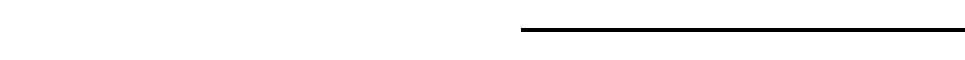
\begin{tikzpicture}
            \Vertex[x=0.5, y=0.5,color=white,opacity=0.5,label=p, size=1, shape=circle]{p}
            \Vertex[x=-1,y=3,color=white,opacity=0.5,label=q, size=1, shape=circle]{q}
            \Vertex[x=2,y=2.5,color=tugreen,opacity=0.5,label=r, size=1, shape=circle]{r}
            \Vertex[x=4,y=4,color=tuorange,opacity=0.5,label=s, size=1, shape=circle]{s}
            \Vertex[x=2.5,y=6.5,color=white,opacity=0.5,label=t, size=1, shape=circle]{t}
            \Vertex[x=5.5,y=1.75,color=white,opacity=0.5,label=u, size=1, shape=circle]{u}
            \Vertex[x=7.5,y=4,color=white,opacity=0.5,label=v, size=1, shape=circle]{v}
            \Vertex[x=7.5,y=6.5,color=white,opacity=0.5,label=w, size=1, shape=circle]{w}
            \Edge[Direct, label=$m_{q \rightarrow r}$](q)(r)
            \Edge[Direct, label=$m_{p \rightarrow r}$](p)(r)
            \Edge[Direct, label=$m_{r \rightarrow s}$](r)(s)
            \Edge[Direct, label=$m_{w \rightarrow s}$](w)(s)
            \Edge[Direct, label=$m_{u \rightarrow s}$](u)(s)
            \Edge[Direct, label=$m_{t \rightarrow s}$](t)(s)
            \Edge[Direct, label=$m_{v \rightarrow s}$](v)(s)
            \draw[line width=0.5 mm] (-2,-1) -- (9.5,-1);
            \Vertex[x=0.5, y=-8.5,color=tuorange,opacity=0.5,label=p, size=1, shape=circle]{p}
            \Vertex[x=-1,y=-6,color=tuorange,opacity=0.5,label=q, size=1, shape=circle]{q}
            \Vertex[x=2,y=-6.5,color=tugreen,opacity=0.5,label=r, size=1, shape=circle]{r}
            \Vertex[x=4,y=-5,color=white,opacity=0.5,label=s, size=1, shape=circle]{s}
            \Vertex[x=2.5,y=-2.5,color=tugreen,opacity=0.5,label=t, size=1, shape=circle]{t}
            \Vertex[x=5.5,y=-7.25,color=tugreen,opacity=0.5,label=u, size=1, shape=circle]{u}
            \Vertex[x=7.5,y=-5,color=tugreen,opacity=0.5,label=v, size=1, shape=circle]{v}
            \Vertex[x=7.5,y=-2.5,color=tugreen,opacity=0.5,label=w, size=1, shape=circle]{w}
            \Edge[Direct, label=$m_{r \rightarrow q}$](r)(q)
            \Edge[Direct, label=$m_{r \rightarrow p}$](r)(p)
            \Edge[Direct, label=$m_{s \rightarrow r}$](s)(r)
            \Edge[Direct, label=$m_{s \rightarrow w}$](s)(w)
            \Edge[Direct, label=$m_{s \rightarrow u}$](s)(u)
            \Edge[Direct, label=$m_{s \rightarrow t}$](s)(t)
            \Edge[Direct, label=$m_{s \rightarrow v}$](s)(v)
            \end{tikzpicture}
    \caption[Two-Pass Belief Propagation on a tree.]{Two pass Belief propagation. In the first pass, messages are collected from the leaves towards the designated root \texttt{s}. White nodes are computed first, then green nodes, and finally, the orange root, that has to wait for node \texttt{r}. In the second pass, the messages are propagated from the root back to the leaves, starting with the white node followed by green nodes and finally orange nodes.}
    \label{fig:beliefprop}
\end{figure}

In the general case, when the graph is not tree-structured, we can employ an approximation algorithm in a similar fashion. 
Loopy belief propagation, as shown in \alg~\ref{alg:lbp} uses a similar approach but has no convergence guarantees.
Instead of reaching guaranteed convergence in two passes, we compute new messages on each vertex by sending old messages back and forth between vertices.
This is done by computing messages in both directions for each edge i.e., 
\begin{equation}
    \begin{split}
        \label{eq:mespas}
        m_{t \rightarrow v}(x_v) &= \sum_{x'_{V_t}} \psi_{vt}(x_v, x_t') \prod_{s\in \mathcal{N}(t) \setminus \{v\}} m_{s \rightarrow t}(x_t) \\
        m_{v \rightarrow t}(x_t) &= \sum_{x'_{V_v}} \psi_{tv}(x_t, x_v') \prod_{u\in \mathcal{N}(v) \setminus \{t\}} m_{u \rightarrow v}(x_v). \\
    \end{split}
\end{equation}

The partition function can then be computed in terms of cumulative messages\cite{piatkowski2018exponential} at any node as 
\begin{equation}
    Z = \sum_{\vect{x} \in \mathcal{X}_v} \prod_{u \in \mathcal{N}(v)} m_{u \rightarrow v}(\vect{x}_v).
\end{equation} 
The resulting partition function is the normalized to the probability distribution with the current parameters $\vect{\theta}$.

\begin{algo}{Loopy Belief Propagation}
    \begin{algorithm}[H]
        \caption{Loopy Belief Propagation}
        \begin{algorithmic}
            \label{alg:lbp}
            \REQUIRE Graph G=(V,E), Model Parameters $\vect{\theta} \in \mathbb{R}^d$, Threshold~$\epsilon > 0$, Number of Iterations $n$\\
            \ENSURE  Node and Edge Marginals $\hat{\mu} \in [0,1]^{d + \abs{V}}$ \\
            \STATE{$\vect{m}^{new} \leftarrow 0, \vect{m}^{old} \leftarrow \infty$}
            \FOR{i=1 ...n}
            \STATE{$\vect{m}^{new} \leftarrow \vect{m}^{old}$} 
                \FORALL{$u,v \in E$}
                \STATE{Update messages $m_{u \rightarrow v}(\vect{x}_v)$ and $m_{v \rightarrow u}(\vect{x}_u)$ (\eq~\ref{eq:mespas})}\\
                \ENDFOR
                \IF{$\epsilon \geq  \abs{\vect{m}^{new} - \vect{m}^{old}}$}
                \STATE{$\vect{m}^{new} \leftarrow \vect{m}^{old}$}\\
                \STATE{BREAK}\\
                \ENDIF
            \ENDFOR
            \RETURN {Normalized messages $\hat{\mu}$~(\eq~\ref{eq:normbp})}
        \end{algorithmic}
    \end{algorithm}
\end{algo}
\subsection{Structure Learning}

So far we have talked about estimating the parameters of exponential family models and performing probabilistic inference.
Determining the structure of a probabilistic graphical model is also a critical task, that needs to be considered when dealing with probabilistic models.
Given a data set $\mathcal{D}$ we associate each dimension of $\mathcal{D}_{\cdot i}$ with a univariate random variable $X_i$, which is then represented as a vertex in the graph.
While the number of vertices is given by the number of features in $\mathcal{D}$, we rarely have explicit information about the conditional independencies between these random variables. 
Therefore, it is necessary to estimate the independence structure, which usually involves finding dependencies between features in $\mathcal{D}$. 
Given a graph $G=(V, \cdot)$ we want to find the subset of edges $E \subset V \times V$, which best represents the underlying independence structure of $\vect{X}$.

Even in case of a predetermined independence structure, we may still aim to either reduce the complexity by removing edges or verify the independence structure.
Various approaches for finding conditional independencies between random variables exist.
Algorithms such as the Chow-Liu algorithm generate a set of conditional independencies such that the resulting graph is a tree.
Other algorithms are less constrained in the choice of edges and generate graphs without guarantees for the final structure.
Chordalysis is one such tool that uses algorithms, which do not necessarily result in a tree-structured graph, which can be used for more complex structures that can not be properly represented as a tree. 
Generally, tree structures are easier to deal with \wrt to training and inference but often yield worse results as they can not capture the proper independence structure, but rather an approximation of the true structure.

For this work, we will focus on tree-structured graphs generated by the Chow-Liu algorithm, which uses a graph weighted by cross-correlation between random variables and minimum spanning trees in order to find the edges, with the highest correlation.
However, the aggregation mechanics are not limited to trees and can be used by any set of parameter sharing the same structure.

\paragraph*{Chow-Liu Algorithm}
Chow and Liu introduced an algorithm~\cite{chow1968approximating} for approximating first order dependency structures using second order terms, where second order terms or probabilities are conditional probabilities conditioned on an additional random variable e.g. $\mathbb{P}(X \lvert Y)$.
The tree is constructed by finding the set of edges that minimizes the Kullback Leibler divergence between the true distribution $\mathbb{P}*$ and the distribution induced by the set of edges $\mathbb{P}_T$, where $T=(V, E_T)$ is a tree.
We obtain the edges by computing the maximum spanning tree on a fully connected weighted graph.
The weights for each edge are based on mutual information between all random variables.

\begin{definition}{Weighted Undirected Graph}
    Let $G=(V,E)$ be a graph, where $E = V \times V$ and let further $c: V \times V \rightarrow \mathbb{R}$ be a cost function associated with edges of G with $c(u,v) = c(v,u) \; \forall u,v \in V$.
\end{definition}

The cost function $c(u,v)$ is the mutual information between two random variables, i.e. 
\begin{equation}
    c(\vect{X}_v, \vect{X}_u) = I(X_v, X_u) = \sum_{\vect{x}_v \in \mathcal{X}_v} \sum_{\vect{x}_u \in \mathcal{X}_u} \mathbb{P}(\vect{x}_v,\vect{x}_u) \log \frac{\mathbb{P}(\vect{x}_v,\vect{x}_u) }{\mathbb{P}(\vect{x}_v)  \mathbb{P}(\vect{x}_u)},
\end{equation}
where the probabilities are usually the relative frequencies of the observed events from $\mathcal{D}$.
Obtaining the minimum Kullback-Leibler divergence is then equivalent to computing the maximum spanning tree on the connected graph as this is the tree that minimizes the Kullback Leibler divergence.
\begin{equation}
    \min_{E_T} KL(\mathbb{P}^*, \mathbb{P}_{E_T}) = \max_{E_T} \sum_{(u,v) \in E_T} c(\vect{X}_v, \vect{X}_u), \; s.t. \; \abs{E_T} = \abs{V}-1 .
\end{equation}

\begin{figure}[!htb]
    \center
        \begin{tikzpicture}
            \Vertex[x=0.5, y=0.5,color=white,opacity=0.5,label=p, size=1, shape=circle]{p}
            \Vertex[x=-1,y=3,color=white,opacity=0.5,label=q, size=1, shape=circle]{q}
            \Vertex[x=2,y=2.5,color=white,opacity=0.5,label=r, size=1, shape=circle]{r}
            \Vertex[x=4,y=4,color=white,opacity=0.5,label=s, size=1, shape=circle]{s}
            \Vertex[x=2.5,y=6.5,color=white,opacity=0.5,label=t, size=1, shape=circle]{t}
            \Vertex[x=5.5,y=1.75,color=white,opacity=0.5,label=u, size=1, shape=circle]{u}
            \Vertex[x=7.5,y=4,color=white,opacity=0.5,label=v, size=1, shape=circle]{v}
            \Vertex[x=7.5,y=6.5,color=white,opacity=0.5,label=w, size=1, shape=circle]{w}
            \Edge[label=\textcolor{black}{$20$}, color=tuorange](q)(r)
            \Edge[label=\textcolor{black}{$17$}, color=tuorange](p)(r)
            \Edge[label=\textcolor{black}{$15$}, color=tuorange](r)(s)
            \Edge[label=\textcolor{black}{$9$}, color=tuorange](w)(s)
            \Edge[label=\textcolor{black}{$3$}, color=tuorange](u)(s)
            \Edge[label=\textcolor{black}{$8$}, color=tuorange](t)(s)
            \Edge[label=\textcolor{black}{$4$}, color=tuorange](v)(s)
            \Edge[label=\textcolor{black}{$2$}, color=tugray](r)(t)
            \Edge[label=\textcolor{black}{$1$}, color=tugray](r)(u)
            \Edge[label=\textcolor{black}{$6$}, color=tugray](q)(t)
            \Edge[label=\textcolor{black}{$3$}, color=tugray](v)(w)
            \Edge[label=\textcolor{black}{$5$}, color=tugray](w)(t)
            \Edge[label=\textcolor{black}{$1$}, color=tugray](u)(v)
            \Edge[label=\textcolor{black}{$5$}, color=tugray](q)(p)
            \Edge[label=\textcolor{black}{$2$}, color=tugray](p)(u)
            \end{tikzpicture}
    \caption[]{Weighted graph G=(V,E), where each weight is the mutual information between two random variables. The edges used for the maximum spanning tree are colored orange, which have a total weight of 76. While the original graph is usually fully connected, some edges have been omitted for better visibility. We assume that the missing edges each have a weight of 0.}
    \label{fig:mst}
\end{figure}

Here connected means, that there exists a path between each pair of vertices in G. 
Such a spanning tree can be found with algorithms such as Prim's or Kruskal's algorithm.
The resulting graph is then guaranteed to be a tree, with edge weights that minimize the Kullback-Leibler divergence between the true distribution and the distribution induced by the tree, i.e., out of all possible sets of edges forming a tree this is the best.

Structure learning is a necessary step before starting parameter estimation as the structure directly affects the number of parameters, the final distribution and without structure, we only have statistically independent random variables. 
The tree is then used on all distributed learners to estimate parameters individually based on the locally observed data. 

Now that we have introduced the necessary tools to create a probabilistic graphical model from a plain data set and estimate parameters for the canonical exponential family, we will move towards bringing these models into distributed learning.


\section{Distributed Learning}
%In the previous sections we explored probabilistic graphical models, inference and structure learning algorithms, which can be used on an arbitrary number of devices.
%Next we will talk about 
With an increasing demand for parallel or distributed programming and learning, caused by more frequently occurring data parallelisms~\cite{ben2006principles}, tasks that were solved on single-core CPUs now more often computed in a distributed environment.

While the increase in CPU performance has diminished over the past few years~\cite{herlihy2011art} due to space and cooling constraints on processors, the amount of individual devices and data collected on these devices has drastically increased~\cite{kaisler2013big}.
Alternatives to centralized machine learning are often found in distributed learning, where the task is split into several smaller tasks, which are then computed in parallel. 
This allows us to increase the efficiency and scalability based on the number of devices available.
However, this approach introduces a necessity for communication between devices since results, data, or updates have to be exchanged.

Our goal in this work is to aggregate probabilistic graphical models received from a set of distributed learners, such that in the end, we are able to create an aggregate model, while not being constrained to a centralized approach.
This method scales well as we can arbitrarily increase the number of learners without being restricted to a single model only.
Performing parameter estimation on distributed learners is straightforward and initially does not change much if each learner estimates their own set of parameters on local data.
First, we need to identify the task and environment we want to apply distributed learning on.
The available data may either be distributed onto different devices or stored at some central server.
Depending on the data distribution and additional constraints such as privacy preservation or constrained communication the chosen approach varies greatly.
Given a data set $\mathcal{D} = \{\mathcal{D}^1, \ldots \mathcal{D}^k\} \subseteq \vect{\mathcal{X}}^m$,
where data chunks $\mathcal{D}^i$ are available on a set of distributed learners.
Recall that we previously introduced horizontally distributed data, which is a subset of the data, such that $\mathcal{D}_{A} = \{\vect{x}^1, \ldots, \vect{x}^A \lvert A \leq n\}$ from state-space $\mathcal{X}^m$ is a subset of samples.

The distributed learners are able to communicate with a coordinator or among each other in a network.

\begin{definition}{Network}
    Let $N = (V, E)$ be a network graph with nodes $V_i, \: i \in I$ over an index $I=\{1,\ldots,k\}$, where each node represents a distributed learner with model $m^{(i)}$ and edges $E$. 
    Existing edges indicate a bidirectional connection between two learners, which allows the connected parties to exchange messages.
\end{definition}

Connectivity between devices in networks may change over time, which requires a more dynamic approach that can deal with frequently changing network structure.
The second approach uses a coordinator node to send or receive updates from distributed learners. 
Most if not all communication is managed by the coordinator, while data may still be kept on the local devices only.
In theory, it is also possible to combine both approaches, i.e., to allow communication between local devices to some degree to achieve a better local solution.
Lastly, in the fully centralized approach, all data is kept on the server is then partitioned into chunks and sent to local devices, which then execute some task, which is for example the case in a Map\&Reduce framework~\cite{dean2010mapreduce}.

Employing a set of distributed learners is useful when the data is horizontally distributed and can not be sent to a central server.
This is the case when there is too much data to process relative to the available bandwidth or when the data contains private information.
Generally, in such instances, it is a good idea to keep communication costs as low as possible as high communication costs only increase the complexity of the overall model.
Statistical models allow for efficient communication as it is sufficient to send the estimated local model parameters $\vect{\theta}^i$ to the coordinator. 

Probabilistic graphical models are compact as we are only required to store the sufficient statistics, the number of samples, model parameters and graph on a distributed learner resulting in a memory complexity of $\mathcal{O}(d + \abs{E})$, where d is the number of parameters and $\abs{E}$ are the number of edges in the graph. 
Already observed and processed data can be safely dropped from memory once the local sufficient statistics are updated.

The two major questions we have to answer in a distributed environment are:
\begin{itemize}
    \item How much data do we need to obtain sufficiently good local models?
    \item How do we aggregate the models once we have obtained the model parameters from local devices?
\end{itemize}

This work primarily focusses on model aggregation, which will be extensively discussed in chapter \ref{chapter:ch3}. 
We will now briefly discuss convergence and sample complexity.

\subsection{Convergence}
Given a set of distributed learners, we want to determine when to stop training the local models and when to stop exchanging model parameters and aggregate the model parameters.
Even more so when memory, processing capabilities, and energy are limited.
We distinguish between two types of convergence criteria, fixed and dynamic.
Fixed convergence is determined at the start of each instance of distributed learners by setting a bound in form of a hyperparameter.
Using such a bound we obtain for example a number of samples required to guarantee this bound and continue training until we have reached this threshold.
Dynamic convergence requires communication between learners or the coordinator, which then monitors some criterion, and if it is fulfilled broadcasts a stopping command to all learners. 

Moreover, each learner needs to determine a local point of convergence at which the learner posts its parameters to other learners or the coordinator. 
This is called the local convergence criterion as opposed to the previously mentioned global convergence criterion.

\paragraph*{Local Convergence}
Local models are trained using gradient descent to minimize the likelihood. 
Recall that the likelihood is convex, thus updates improve upon the objective, towards the global minimum.
As $\vect{\theta}$ moves towards the global minimum and with appropriate step-size the difference between two subsequent objective function values decreases.
Hence, we may use this difference as a method to determine convergence, given some threshold $\varepsilon$ we stop the optimization if the different between two likelihoods falls below this threshold, i.e.:
\begin{equation}
    \abs{\ell(\vect{\theta}^{(t+1)} ; \mathcal{D}) - \ell(\vect{\theta}^{(t)} ; \mathcal{D})} \leq \varepsilon,
\end{equation}
where the choice of $\varepsilon$ determines how small the likelihood rate of change has to be before terminating the training.
Note, that $\theta^t$ here denotes the t-th iteration instead of the parameters on the t-th local device.
When the gradient is close to zero, we may also terminate the optimization as the optimum is located at $\nabla_{\vect{\theta}} \ell(\vect{\theta}^{*} ; \mathcal{D}) = 0$ and once the gradient
\begin{equation}
    \norm{\nabla_{\vect{\theta}} \ell(\vect{\theta}^{(t)} ; \mathcal{D})}_{\infty} \leq \epsilon
\end{equation}
is sufficiently close to zero we terminate the optimization. 

Alternatively, we may always train each model for a predetermined number of iterations without explicit stopping criterion.

\paragraph*{Global Convergence}

Data on the distributed learnings grows dynamically over time.
On each device is dynamically accumulated, i.e. new data is observed in each round, where a each starts in a synchronous fashion on all learners.
At the start of each round, every learner first checks if there are new samples available and extends the local sufficient statistics by the newly observed samples.
This can be accomplished by keeping a record of the sufficient statistics and the number of samples observed.
The new sufficient statistics at round $t+1$ are then the weighted average of the old average sufficient statistics and time $t$ and new observations 
\begin{equation}
    \vect{\tilde{\mu}}^{t+1} = \frac{\abs{\mathcal{D}^{t}}\vect{\tilde{\mu}}^t + \sum_{\vect{x} \in \mathcal{D}^{new}} \phi(\vect{x})}{\abs{\mathcal{D}^{t}} + \abs{\mathcal{D}^{new}}}.
\end{equation}

However, the already observed data is still incorporated in the sufficient statistic and only changes depending on the number of new samples discovered.
If the sufficient statistic does not change much, e.g. when we already have a large number of samples and only observe a small amount of new data, the objective is not likely to change too much. 
Instead of simply restarting the training, we can check if the old parameters on the i-th learner are still sufficiently close to the optimum in terms of the new data: 

\begin{equation}
    \norm{\nabla_{\vect{\theta}^t} \ell(\vect{\theta}^{t} ; \mathcal{D}_i^{t+1})}_{\infty} \leq \epsilon,
\end{equation}
then choose to omit training, if the gradient is still $\epsilon$-close to zero.

The total memory requirement is linear in the number of parameters, that is, the d-dimensional space that $\phi$ maps to, thus each model only requires $\mathcal{O}(d)$ memory.
Using this iterative approach we can keep track of the number of samples observed and the current state of the model.
Now, we need to determine a stopping criterion, which allows us to terminate the optimization and data gathering process if so desired. 
Otherwise, we may also choose to keep the optimization and data acquisition running indefinitely in case we expect new observations to vary, such that the underlying distribution changes.

We then have to devise a suitable evaluation mechanism, that allows us to define a stopping criterion based on criteria such as the amount of data observed or some distance measure between parameters or sufficient statistics on distributed learners.

\subsection{Bounds on Sample Complexity and Variance}
\label{ssec:bounds}
One of the key questions of distributed learning is the number of samples required to obtain local models that are sufficiently good, i.e., when to stop gathering new data.
This also implies having knowledge of when the model is good enough to stop training.
The problem to find the number of samples required cannot be solved exactly, but some bounds exist that allow an estimate of the model quality.
One such bound on the sample complexity is the Hoefding-Bound, which provides an upper bound on the distance between sufficient statistics.
 
We apply the Hoefding-Inequality on the pairwise difference between average sufficient statistics of local models.
Furthermore, we are going to demonstrate that the variance on entries in the sufficient statistics and between the parameters of different models is bounded in the number of samples observed.

First, the Hoefding-Inequality is given by
\begin{equation}
    P(\vect{\bar{X}} - \mathbb{E}[\vect{\bar{X}}] \geq t ) \leq \exp^{-2\abs{\mathcal{D}]t^2}},
\end{equation}

where for some constant $t$ the probability of the difference between the empirical mean of a random variable and its expectation is being greater than $t$ is negatively exponential bounded by the amount of data seen.

Piatkowski~\cite{piatkowski2019distributed} has shown that for $t = \frac{\sqrt{(c+1) \log d}}{2\abs{\mathcal{D}}}$ the difference between two average sufficient statistics $\vect{\mu}^i = \frac{1}{\mathcal{D}_i} \sum_{x \in \mathcal{D}} \vect{\phi(x)}, \; \vect{\phi(x)} \in \mathbb{R}^d$ of a probabilistic graphical model is bounded by
\begin{equation}
    \label{eq:hoefd}
    \norm{\mu^{i} -  \mu^{j}}_\infty \leq 2 \sqrt{
        \frac{(c+1) \log d}
        {2\abs{\mathcal{D^{'}}}}
        } = \epsilon,
\end{equation}

with probability of at least $\delta= (1- 2 \exp(-c \log d))$. Here $D^{'} = \min(\abs{\mathcal{D}^i}, \abs{\mathcal{D}^j})$.

As the average sufficient statistics approach each other, we can show by Popoviciu's Theorem \cite{popoviciu1935equations} that the variance between sufficient statistics $Var[\norm{\vect{\mu}^{i} -  \vect{\mu}^{j}}_\infty]$ is bounded \wrt the max-norm $\norm{\cdot}_{\infty}$.
\begin{threm}{Upper Bound on the Variance}
    Let $\vect{X}$ be a bounded random variable with $\inf(\vect{X}) = b$ and $\sup(\vect{X}) = a$, 
    then the variance $Var[\vect{X}] = \sigma^2$ is bounded by 
    \begin{equation}
        \sigma^2 \leq \bigg(\frac{a-b}{2}\bigg)^{2}
    \end{equation}
\end{threm}

Results by Sharma et al. \cite{sharma2010betterbounds} suggest a slightly improved bound by using the third central moment.
However, we consider the upper bound defined by Popoviciu to be sufficient in this case.

\begin{proof}{Bound of Variances}

Let $f(t) = \mathbb{E}[(\vect{X} - t)^2]$ for some $t$ and $b = \inf(\vect{X})$, $a = \sup(\vect{X})$ for a bounded random variable $\vect{X}$.

The derivative of $f(t)$ is:
\begin{equation*}
    \begin{split}
        f'(t) &= \frac{d}{dt} \mathbb{E}[(\vect{X} - t)^2]\\ 
            &= -2\mathbb{E}[\vect{X}] + 2t = 0\\
    \end{split}
\end{equation*}
and takes its minimum at $t = \mathbb{E}[X]$, which is $f(\mathbb{E}[X]) = \mathbb{E}[(\vect{X} - \mathbb{E}[X])^2] = Var[X]$ the variance of the random variable.

Now let  $t=\frac{a-b}{2}$, the arithmetic mean $\sup(\vect{X})$ and $\inf(\vect{X})$, which maximizes the distance between $t$ and $a,b$.
We obtain the following inequalities for the maximizer:

\begin{equation*}
    Var[\vect{X}] = f(\mathbb{E}[\vect{X}]) = \mathbb{E}[(\vect{X} - \mathbb{E}[\vect{X}])^2) \leq f(\frac{a-b}{2})
\end{equation*}

with 

\begin{equation*}
    f\bigg(\frac{a-b}{2}\bigg) = \mathbb{E}\bigg[\bigg(\vect{X} - \frac{a-b}{2} \bigg)^2\bigg]= \frac{1}{4} \cdot \mathbb{E}\bigg[\big((\vect{X} - b) + (\vect{X} - a)  \big)^2\bigg]
\end{equation*}

We then have 
\begin{equation*}
         \bigg((\vect{X} - b) + (\vect{X} - a)  \bigg)^2 \leq  \bigg((\vect{X} - b) - (\vect{X} - a)  \bigg)^2  = (a-b)^2 
\end{equation*}
We now show that the equality on the right hand side holds.
Let $\vect{X} = a - \epsilon, \quad \epsilon \in [b,a]$ : 

\begin{equation*}
    \begin{split}
        \bigg(((a-\epsilon) - b) - ((a-\epsilon) - a)  \bigg)^2  &=  (a-b)^2\\
        \bigg(((a-\epsilon) - b) + \epsilon  \bigg)^2 &=  (a-b)^2 \\
        (a-b)^2  &= (a-b)^2,\\
    \end{split}
\end{equation*}
\qed
thus for any $\epsilon \in [b,a]$ the equality holds.

For the expected value of $\vect{X}$ we then have
\begin{equation*}
    \frac{1}{4} \cdot \mathbb{E}\bigg[\big((\vect{X} - b) + (\vect{X} - a)  \big)^2\bigg] \leq \frac{1}{4} \cdot \mathbb{E}\bigg[\big((\vect{X} - b) - (\vect{X} - a)\big)^2\bigg] = \bigg(\frac{a-b}{2}\bigg)^2,
\end{equation*}\qed
obtaining the following bound on the variance of a bounded random variable:
\begin{equation}
    Var[\vect{X}] = \sigma^2 \leq \bigg(\frac{a-b}{2}\bigg)^2
\end{equation}
\qed
\end{proof}


Recall that $\norm{\vect{\mu}^{i} -  \vect{\mu}^{j}}_\infty \leq  \epsilon$, where $\epsilon$ is the bound on the largest absolute difference between two entries of the average sufficient statistics. 
Then for some $k$ let  $\mu^{i}_k - \mu^{j}_k = a - b  = \epsilon$ that satisfies the bound with equality.
This means that there exists a no larger difference between entries of the two vectors resulting in an upper bound for the variance of the average sufficient statistics with $a - b = \epsilon$ and thus
\begin{equation*}
    Var[\vect{\mu}^{i}_k -  \vect{\mu}^{j}_k] \leq \frac{\epsilon^2}{4} = \sigma^2 \quad \forall i,j,k.
\end{equation*}
Given two average sufficient statistics, we can employ the Hoefding bound to guarantee the distance and variance between these two to be smaller than some $\epsilon$ with probability $\delta$

Likewise, there is an explicit relationship between the sufficient statistics, sample size, and the model parameters, as shown by Bradley et al. \cite{bradley2012sample}, who consider the MLE bound \wrt to the sample size. 
Let $C_min \geq 0$ be a bound on the smallest eigenvalue of the Fisher information obtained from the true parameters $\vect{\theta}^*$ and $\phi_{max}$ be the maximum magnitude of the sufficient statistics. 
Bradley et al. have shown that \wrt to these parameters the $\ell_1$-norm between the true parameters and some estimate is bounded by 

\begin{equation}
    \label{eq:pac-bound}
    \norm{\vect{\hat{\theta}}- \vect{\theta}^*}_1 \leq \frac{C_{min}}{4r\phi^3_{max}} \abs{\mathcal{D}}^{-\alpha/2},
\end{equation}
where $\alpha$ is a hyperparameter $0 < \alpha \leq 1$ the controls the convergence rate in a trade-off for the probability that this bound holds. 
Rearranging \eq~\ref{eq:hoefd} we substitute $\abs{\mathcal{D}}$ from \eq~\ref{eq:pac-bound} and can show that the distance between the estimate and true parameters is related to the hoefding bound on sufficient statistics
\begin{equation}
    \norm{\vect{\hat{\theta}}- \vect{\theta}^*}_1 \leq \frac{C_{min}}{4r\phi^3_{max}} \frac{\sqrt[2/\alpha]{2\sigma^2}}{\sqrt[2/\alpha]{((c+1) \log d)}},
\end{equation}
where $r < d$ when using the overcomplete representation of sufficient statistics.
We can obtain $r$ from the number of nonzero eigenvalues of the Hessian.

Applying the triangle inequality to the parameters we obtain for any two parameter vectors $i,j$
\begin{equation}
    \norm{\vect{\theta}^i- \vect{\theta}^j}_1 \leq  \norm{\vect{\theta}^i - \vect{\theta}^*}_1  +  \norm{\vect{\theta}^j- \vect{\theta}^*}_1 \leq 2 \frac{C_{min}}{4r\phi^3_{max}} \frac{\sqrt{2\sigma^2}}{\sqrt{((c+1) \log d)}}
\end{equation}
and by the decreasing monotonicity of p-norms \cite{raissouli2010various} we have

\begin{equation}
    \norm{\vect{\theta}^i- \vect{\theta}^j}_{\infty}  \leq \norm{\vect{\theta}^i- \vect{\theta}^j}_1.
\end{equation}

As the amount of data on each device increases, we can also measure how close the sufficient statistics are with probability $\delta$ by rearranging the above equation. 
This is the most common scenario in distributed learning. 
As time progresses, the amount of data increases allowing us to continuously measure the distance and variance between the sufficient statistics.
Once we reach our predetermined goal on a device, i.e. $\abs{\mathcal{D}}^i$ is sufficiently large to satisfy the bound we stop collecting more data send the parameters to the coordinator node.

For a given probability $\delta$ and with variance threshold $\sigma^2 = (\epsilon/2)^2$ we rearrange \eq~\ref{eq:hoefd} to obtain 
\begin{equation}
    \abs{\mathcal{D}} = \frac{(c+1) \log d}{2 \sigma^2},
\end{equation}

which is the amount of data necessary to a have variance of at most $\sigma^2$ with probability $\delta$.

We see that as $\abs{\mathcal{D}}$ increases, for a fixed $\delta$ the distance $\epsilon$ decreases and so does the variance. 
In conclusion, we have shown that as the sample size increases the variance for the average sufficient statistics and in turn for model parameters decreases.
This allows us to choose a variance or distance threshold and obtain the necessary amount of data to reach that threshold.

Next, we will introduce methods for sampling from a generative model, which is one of the main advantages these types of models have over discriminative ones.

\section{Sampling}
\label{sec:sampling}
Statistical models such as probabilistic graphical models belong to the class of generative models.
These types of models allow not only for solving discriminative tasks such as classification, but also have the ability to sample new data.
Furthermore, we may observe a learner generating incomplete data with missing entries.
We can perform inference using the model to complete these samples in order to obtain fully observed data.
This is usually based on the configuration with the highest likelihood given the seen entries of a sample.

How do we sample from such a distribution? There are several different ways to sample from such a distribution, two of those are the Perturb and MAP approach and Gibbs sampling.


\subsection{Perturb and MAP}
\label{ssec:pmap}
Recall from \eq\ref{eq:map} that the sample that maximizes the posterior probability is the sample that maximizes the likelihood.
Perturb and MAP (\alg~\ref{alg:pmap}) presents a technique obtaining samples using the maximum a-posteriori probability of a distribution.
The core idea is to add a small amount of noise $\epsilon$ to the model parameters $\vect{\theta}$ effectively changing the mode of the distribution, which leads to a different maximizer for the a-posteriori probability. 
\begin{equation}
    \hat{\vect{x}}  = \arg\max_{\vect{x} \in \vect{\mathcal{X}}} \mathbb{P}_{\vect{\theta}}(\vect{x})
\end{equation}

We then sample $\epsilon$ from an arbitrary probability distribution to perturb the model parameters
\begin{equation}
    \hat{\vect{x}}  = \arg\max_{\vect{x} \in \vect{\mathcal{X}}} \mathbb{P}_{\vect{\theta} + \epsilon}(\vect{x}), \quad \epsilon \sim f(x),
\end{equation}
where $\epsilon \sim f(x)$ may for example be a normal distribution.

Now consider the asymptotic normality of exponential families as well as the bound on variances. 
We can use both in such a way that $\epsilon\sim \mathcal{N}(0, i(\vect{\theta}^*)/n)$ is a sample from a normal distribution with variance based on the asymptotic normal distribution, which allows us to sample an error within the natural error range.
This way we can sample from different MAP-States, while still accounting for the error of the current parameters \wrt to the true parameters.


\begin{algo}{Perturb and MAP~\cite{papandreou2011perturb}}
    \begin{algorithm}[H]
        \caption{Perturb and MAP}
        \begin{algorithmic}[1]
            \label{alg:pmap}
            \REQUIRE Sample Probability Distribution $\mathbb{P}_{\vect{\theta}}$, Perturb Distribution $\mathbb{Q}_{\vect{\lambda}}$
            \ENSURE  MAP-State $\hat{\vect{x}}$ from $\mathbb{P}_{\vect{\theta} + \epsilon}(\vect{x})$ \\
            \STATE{Sample $\epsilon \sim \mathbb{Q}_{\vect{\lambda}} $}\\
            \STATE{$\hat{\vect{x}} \leftarrow \arg\max_{\vect{x} \in \vect{\mathcal{X}}} \mathbb{P}_{\vect{\theta} + \epsilon}(\vect{x})$}\\
            \RETURN {$\hat{\vect{x}}$}
        \end{algorithmic}
    \end{algorithm}
\end{algo}

\subsection{Gibbs Sampling}
The Gibbs Sampling algorithm as presented in \alg\ref{alg:gibbs} is another method of obtaining samples $\vect{x} \in \vect{\mathcal{X}}$ from a probability distribution. 
Initially, we sample from a uniform distribution in the range $[0,1]$ and then proceed to compute the marginal probabilities for a single entry and replacing that entry with the most probable one.
This is repeated for randomly chosen elements and it can be shown that the initially uniform sample asymptotically approaches the actual distribution.
However, as this may be computationally inhibitive due to the iterative nature of this method we may stop after a certain number of iterations, obtaining a sample which is approximately from the distribution of $\vect{X}$.

\begin{algo}{Gibbs Sampling~\cite{yildirim2012bayesian}}
    \begin{algorithm}[H]
        \caption{Gibbs Sampling}
        \begin{algorithmic}[1]
            \label{alg:gibbs}
            \REQUIRE $\vect{x} \sim f(\tau) \in \mathbb{R}^m$, Graph G=(V,E)
            \ENSURE  $\vect{x} \sim \mathbb{P}_{\vect{\theta}}\in \mathbb{R}^m$ \\
            \FOR{i=1 ...n}
                \FORALL{$j \in V$}
                \STATE{$x_j \leftarrow x_j \sim \mathbb{P}_{\vect{\theta}}(\vect{X}_j = x_j \lvert \mathcal{N}(\vect{X}_j) )$}
                \ENDFOR
            \ENDFOR
            \RETURN {$\vect{x}$}
        \end{algorithmic}
    \end{algorithm}
\end{algo}
